\chapter{6. Conclusion}

\section{Future Work}
\label{sec:future}

\subsection{collective urban planning tool kit}

While it will be useful to have a general application that goes beyond reporting and enables users to propose an intervention,
there is a risk that it will be difficult to maintain the attention for one mobile application.
An alternative is to create a framework of the application, which can be customized to specific
targets similar to bike lane security and topics discussed in the DISCUSSION section.


Recent web application developments have focused on how to handle and create modular parts to make it easy to reuse and distribute. We can observe this by NPM (Node Package Manager)
\footnote{A software that automates dependency checking and installing parts of software to be used in combination.}
There are more than 475,000
\footenote{\url{https://www.npmjs.com/}}
building blocks that one can combine to make web based applications. The elements of one application are modular as well, were one application is components combined together.

A possible next step for bikebump is a set of reusable components that could be reconfigured to track other urban issues, like collectively change speed limits\footenote{in both ways}, changing the frequency of street lights, or zoning.


\subsection{safer route navigation}
Utilizing the data collected by the users, we can make a routing system based on safeness within the roads.

Modern map services enable custom path finding, where applications can set different weights for each road segment. Improving the overall bike experience will introduce people to ride their bikes more frequently, reducing use of cars on crowded urban streets. 
The ring bell Geo location data having weights good and bad, the paths can be altered to take a safer route.
This will incentivize the users for using the application. In addition, the reported data can be sourced to car navigation systems to let car drivers notice places that are bike-heavy.


\subsection{inclusive design for non-bikers}

\begin{marginfigure}[{2cm}]
 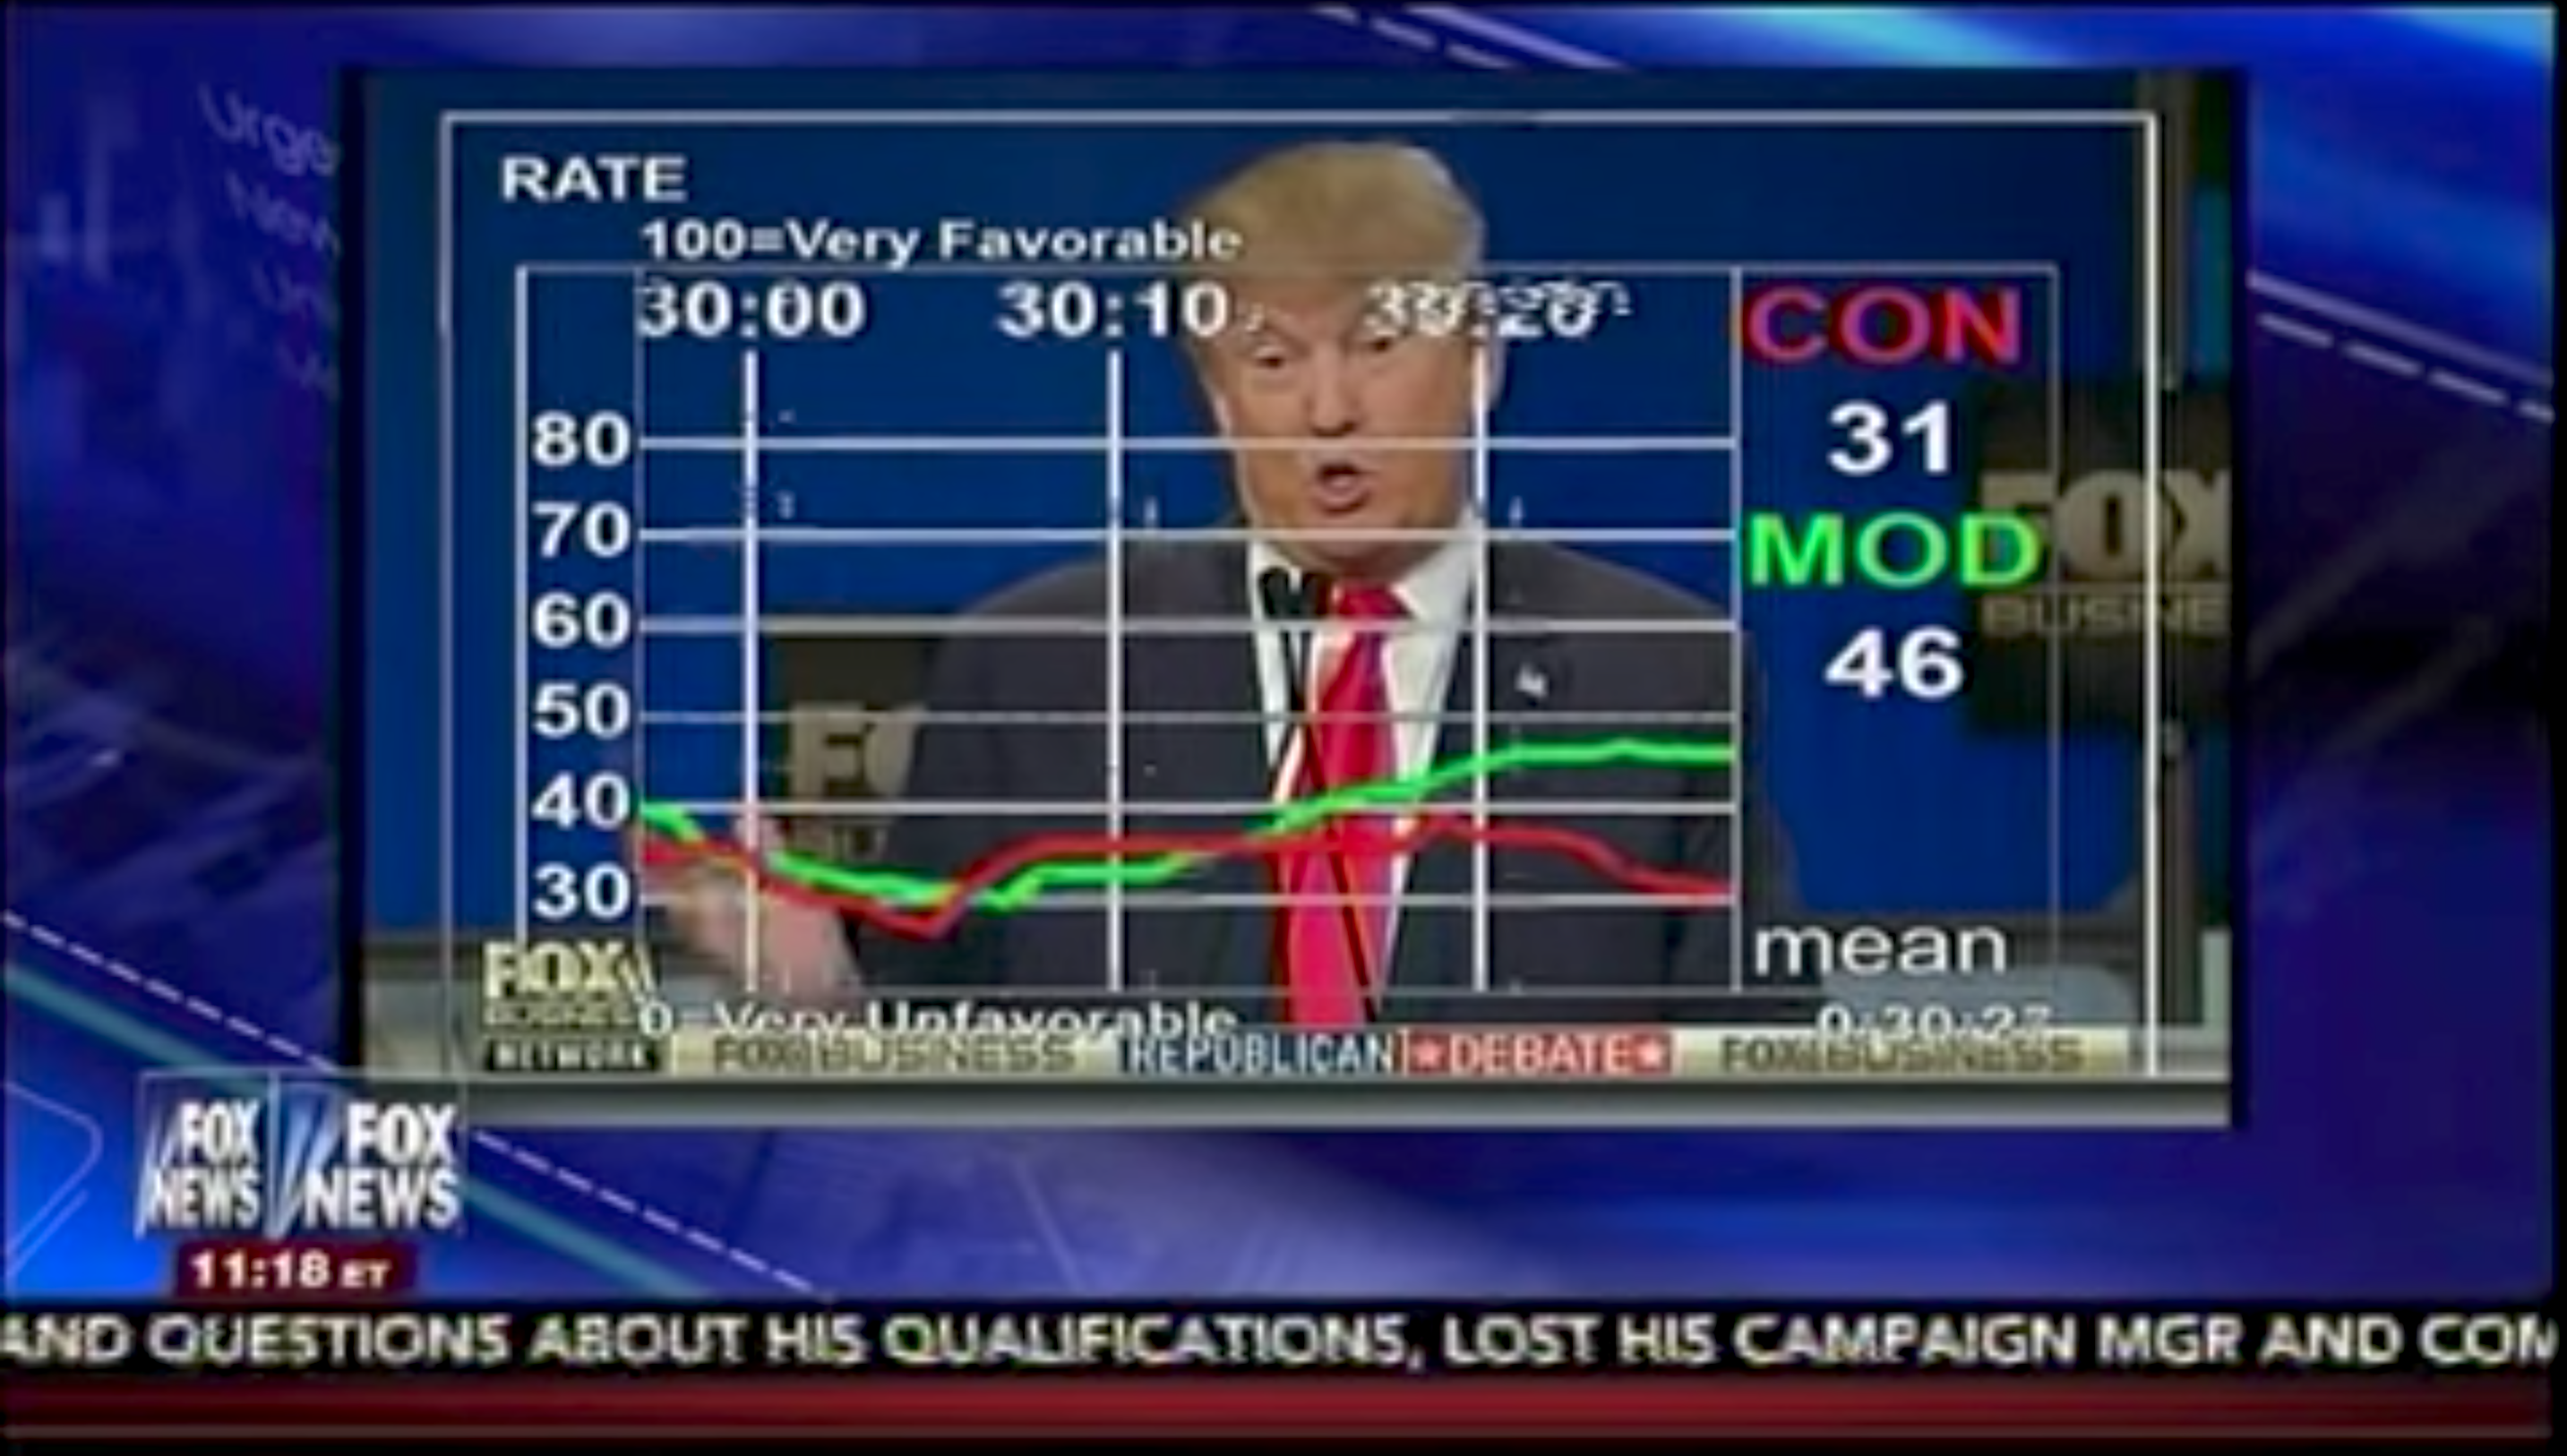
\includegraphics[width=\textwidth]{chapters/6/fig/pollester.png}  \caption{method for continuous input}
 \label{fig:poll}
\end{marginfigure}
This app had focused on bikers, and did not take into account people who use other modes of transportation, such as pedestrians or car drivers. It is important to incorporate input from diverse people, and this both applies to the analytical and synthetic phase. It is easy to imagine to discuss the prioritization side, but the data on on-bike reports be should capture in a simulated environment.
Using a VR headset can simulate the bike ride and solicit data from people using a virtual environment projecting recorded material of one commute. \hlcyan{In this case, it will be harder for people to explore proactively, so the city may have to define an area of concentration, and have people who uses the road but with other modes of transportation validate weather the data is not over weighted to bikers. Very inexpensive headsets such as Google's cardboard or day dream may be used for scaling.\footnote{ \url{https://vr.google.com/}} In addition video footage from 360 camera could be used for supplement visual reality.}

\subsection{Incentivasation}
In the discussion section, further considerations were are necessary for the synthesis phase because of the time difference of the proposal and execution; people may not be able to benefit what they asked.

The easiest way is to provide a cash incentive for individuals who proposed according to the number of votes that were collected through that app. In fact, this is an act of planning nothing different to a planner. 
To do this, we would first need to convert the BIKE COIN tokens into currency that is reasonably transferable to money. The BIKE COIN token may be remain entirely in side the system, yet if it proves to make certain change there is possibility that will be treated as currency as we see in MMORPGs. In this way we can weight the influence according to the previous effort and reputation the user had made.
Another method may be indirect cash incentives. First having a public charity fund that entities can put money into, that can be distributed when there is particular collective action. For example, the app might have a corporate sponsor, and the sponsor may give charity to other parts of the world that need when people propose or votes for plans. Individuals may set preferences to where or who to support, in that way the corporate sponsor will be able to know where the people's interest.


\section{Concluding Remarks}

\hlcyan{This thesis explored the possibility of a collective urban design tool by looking into 
one case study of bike way improvements plans.

The thesis started to examine the origin of direct democracy and the physicality of it.
It proceeded to look into what kind of problems planners face today, and how a bottom up
tool would help the procedure for both the planners and the general public.

Examples showed that there is only few mobile based tools that
integrated the analytic and syntactical planning process. Existing methods
concentrated on either of the processes but not to combine them. They were
also focused to collect unstructured data that is often difficult to convert into
an actionable plan.
The study then moved to building a prototype and conducted an
experiment to test the method. The analytic side show that it covered most of the 
bike accidents that occurred through the fixed route, while there is more investigation is
needed for combining urban sound classification techniques. The synthetic 
side showed that most of the users recognized the difference of the two phases,
and mentioned that this might be practical tool for practical uses. 
The thesis then overview what is required to make collective tool
providing a potential to combine the app with the recent thinking of
share economy and ownership.
}



